\chapter{Implementación de hardware}
En este capítulo se detallara cual es el hardware utilizado para el desarrollo del sistema de acceso, se indicarán cuales
son los requisitos mínimos que deben satisfacerse para que el sistema cumpla las características solicitadas, como
también se indicarán los sensores y equipos auxiliares usados junta con otras posibles opciones encontradas y las
razones por las que estas fueron descartadas.


\section{Estado actual del sistema de acceso por barreras}

\subsection{Sistemas tradicionales}

Hoy en día el sistema de uso de barreras para el control de ingreso y egreso a distintos recintos suelen generar molestias
en muchos de los usuarios, por la necesidad de realizar alguna acción extra, con esto nos referimos a la necesidad de
en muchas ocasiones de obtener y guardar algún tipo de ticket, este sistema lo vemos en la Fig. \ref{fig:sistema-tradicional}
 que en caso de perderlo se tenga que pagar una multa económica, o bien de acercarse a un determinado lugar para poder realizar el pago por el tiempo de permanencia.

En este tipo de metodologías es donde queremos realizar un aporte a la reducción del impacto ecológico, ya que si se quita
la necesidad de imprimir uno o más tickets por cada vehículo que ingresa, se estaría disminuyendo considerablemente la
necesidad de utilizar papel y considerando que el método de impresión de estos tickets suele ser por impresión térmica,
proceso donde se utiliza un papel termosensible que al ser calentado se vuelve negro, que tiene un costo electrico
adicional.
\begin{figure}
    \centering
    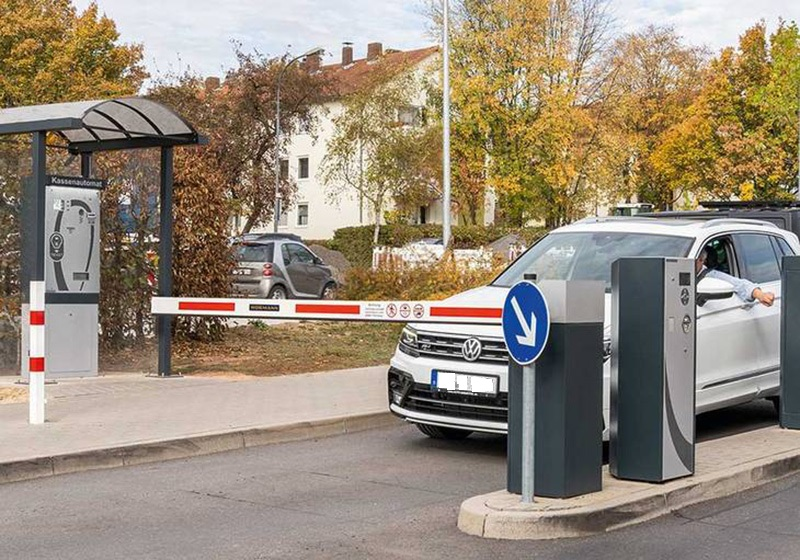
\includegraphics[width=0.5\textwidth]{imgs/sistema-control-acceso-barreras.jpg}
    \caption{Sistema tradicional de acceso por barreras por sistema de pulsador y ticket.}
    \label{fig:sistema-tradicional}
    %%https://www.aradock.es/nuevos-sistemas-de-control-de-accesos-barreras/
\end{figure}

Otro de los aspectos que destacan del uso actual del sistema de barreras en sistemas más manuales es la necesidad de
contar con  operarios trabajando en la barrera el tiempo que la barrera esté disponible, ya que en caso de no disponerlo
deberá quedar la barrera sin efecto, perdiendo por completo su utilidad.

\subsection{Sistemas Modernos}

Con el avance y el abaratamiento de los costos en la electrónica surgieron nuevos métodos que permitieron a los usuarios
prescindir de la necesidad de un ticket o una tercera persona que les facilite el acceso, el método principal es el uso
de controles remotos que al ser accionados, activan el mecanismo y abren el paso del vehículo.
 
Otro sistema que está ocupando gran parte del mercado en los últimos años es el que integra a la barrera un sistema de
RFID, que mediante la colocación de un emisor RF en el vehículo, Fig.\ref{fig:sistema-moderno} o por el método de tarjetas o coins de proximidad y un
receptor en la barrera, al acercarse al ingreso se produce en el enlace que habilita o no al vehículo a ingresar.

\begin{figure}
    \centering
    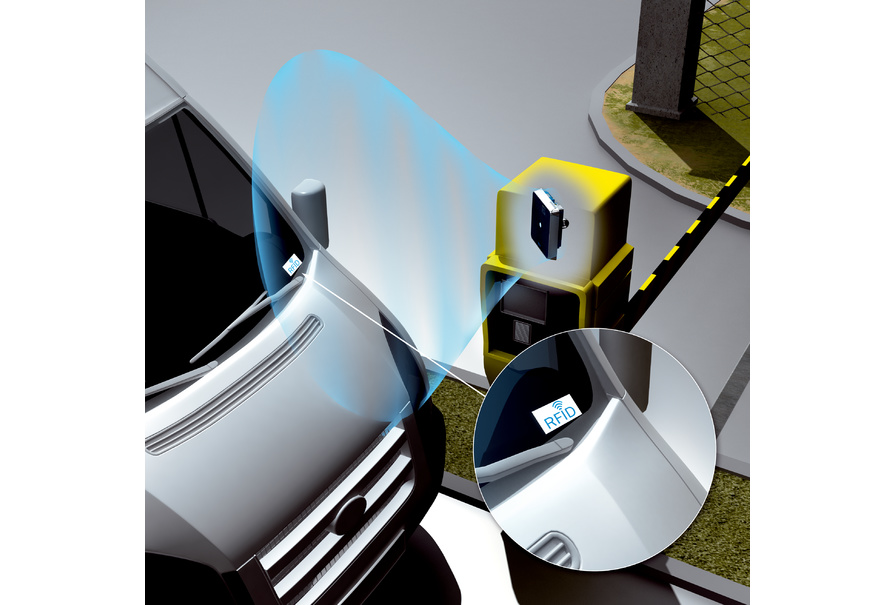
\includegraphics[width=0.8\textwidth]{imgs/sistema-control-acceso-barreras-rfid.jpg}
    \caption{Sistema moderno de acceso por barreras por sistema de RFID.}
    \label{fig:sistema-moderno}
    %%https://www.sick.com/mx/es/sectores/seguridad-de-los-edificios/seguridad-en-los-exteriores/control-de-acceso/acceso-sin-contacto-a-barreras-mediante-rfid/c/p360565
\end{figure}

Todos estos  metodos son muy utiles y agilizan el transito por la zona de entrada que suele rondar entre los 15 y 20 segundos por 
auto,pero tambien presentan la necesidad de contar con algun dispositivo o elemento externo para que este funcione, la finalidad
de este trabajo es obtener un metodo que reduzca el tiempo de ingreso lo maximo posible y retirar la necesidad de elementos
extras, es pocas palabras que solo con la proximadad del automovil sea posible accionar la barrera.

Entonces ¿Que requisitos debe tener el sistema para cumplir lo planteado?, en primera instancia y como el eje del trabajo
es utilizar un algoritmo de OCR, el hardware debe permitir el uso de una camara de al menos una resolucion de 480p, debe 
soportar protocolos de comunicacion (i2c,spi o UART) para el acople de sensores auxiliares necesarios, permitir conexion
etherner/wifi, soporte para el uso de Python3.

\section{Selección de placas}
Teniendo en cuenta los requisitos minimos planteandos en la seccion anterior, surgieron varios opciones posibles 

\section{Evalución y selección de sensores}

\section{Consumo energetico}

\section{Diseño y ensamble}